\section{Установка CentOS 6} \label{pril:a}

\begin{figure}[ht]
    \centering
	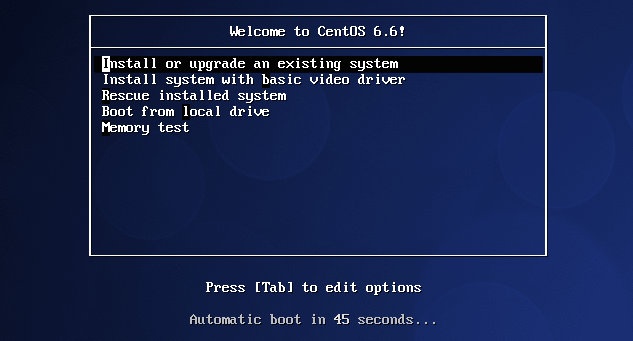
\includegraphics[width=0.8\linewidth]{0}
	\caption{Меню выбора загрузки с носителя}
\end{figure}

\begin{figure}[ht]
    \centering
	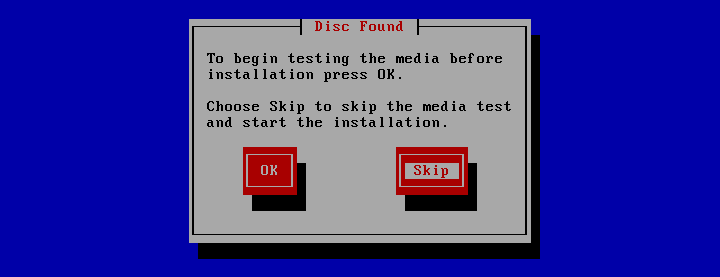
\includegraphics[width=0.8\linewidth]{1}
	\caption{Предложение установщика проверить на ошибки носитель}
\end{figure}

\begin{figure}[ht]
    \centering
	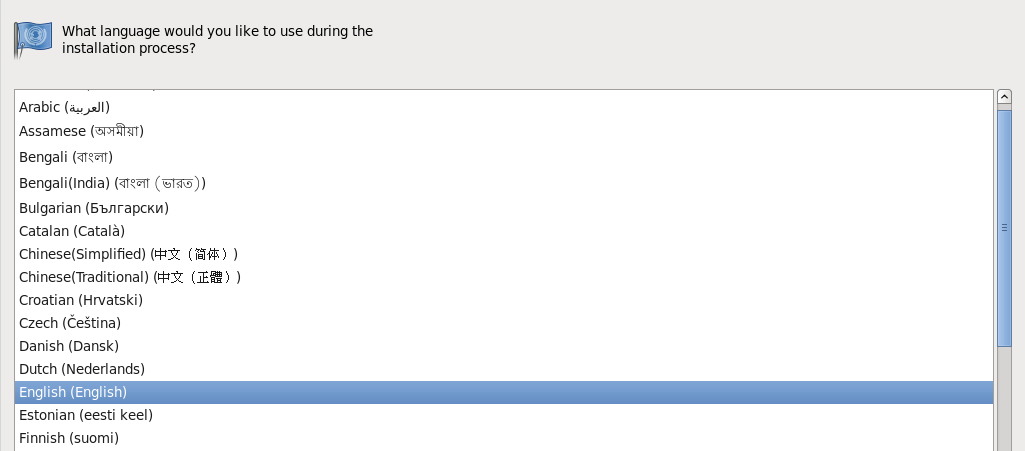
\includegraphics[width=0.8\linewidth]{3}
	\caption{Выбор языка установки}
\end{figure}

\begin{figure}[ht]
    \centering
	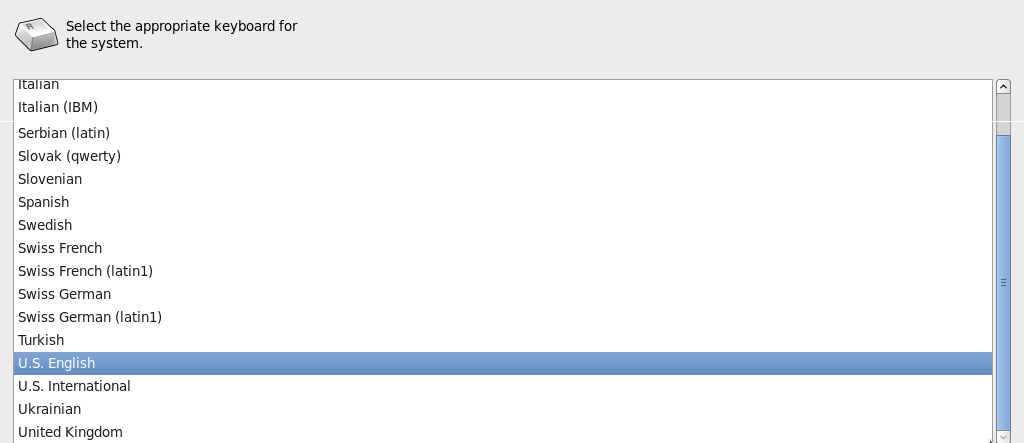
\includegraphics[width=0.8\linewidth]{4}
	\caption{Выбор языковой раскладки клавиатуры}
\end{figure}

\begin{figure}[ht]
    \centering
	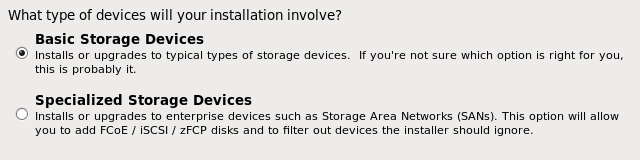
\includegraphics[width=0.8\linewidth]{5}
	\caption{Проверка наличия специализированных устройств}
\end{figure}

\begin{figure}[ht]
    \centering
	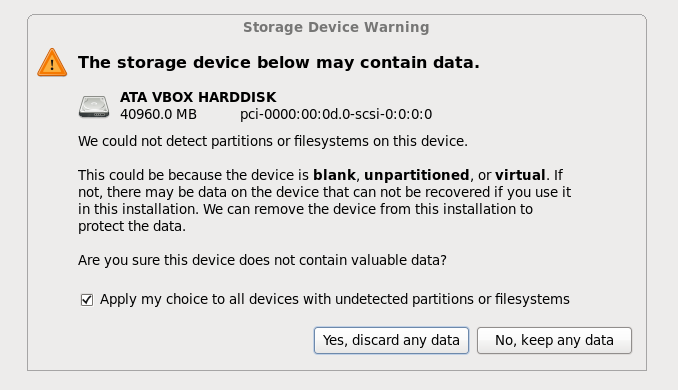
\includegraphics[width=0.8\linewidth]{6}
	\caption{Проверка наличия данных на жестком диске}
\end{figure}

\begin{figure}[ht]
    \centering
	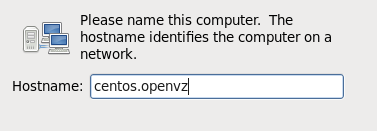
\includegraphics[width=0.8\linewidth]{7}
	\caption{Задание имени компьютера (hostname)}
\end{figure}

\begin{figure}[ht]
    \centering
	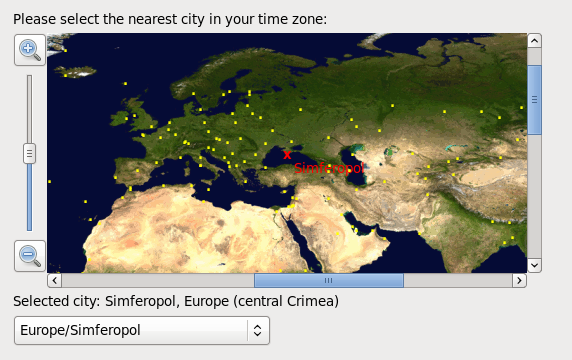
\includegraphics[width=0.8\linewidth]{8}
	\caption{Выбор часового пояса}
\end{figure}

\begin{figure}[ht]
    \centering
	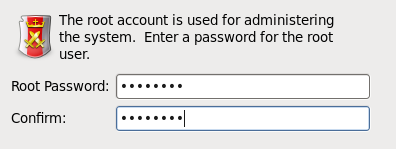
\includegraphics[width=0.8\linewidth]{9}
	\caption{Задание пароля суперпользователя}
\end{figure}

\begin{figure}[ht]
    \centering
	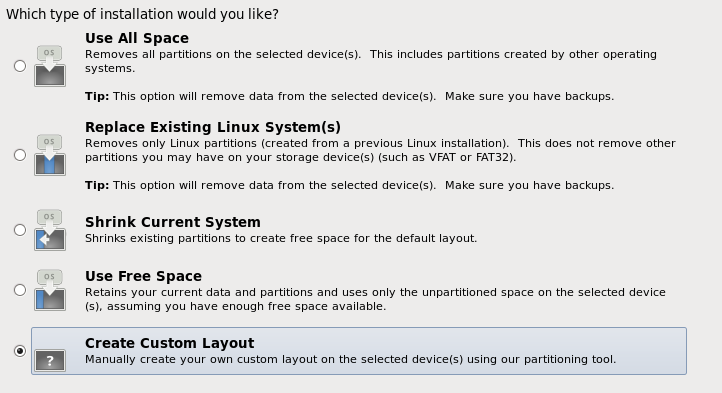
\includegraphics[width=0.8\linewidth]{10}
	\caption{Выбор типа разделения жесткого диска}
\end{figure}

\begin{figure}[ht]
    \centering
	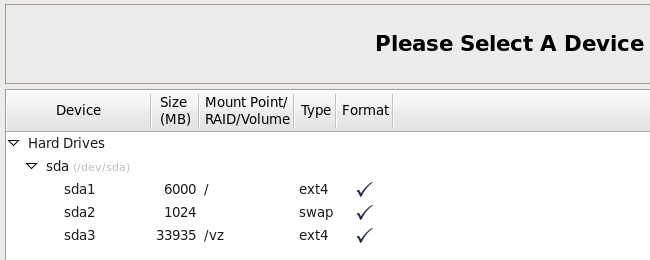
\includegraphics[width=0.8\linewidth]{11}
	\caption{Разметка жесткого диска}
\end{figure}

\begin{figure}[ht]
    \centering
	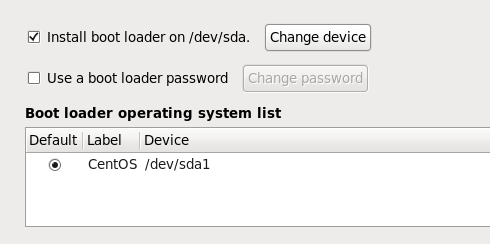
\includegraphics[width=0.8\linewidth]{13}
	\caption{Установка загрузчика}
\end{figure}

\begin{figure}[ht]
    \centering
	
\includegraphics[width=0.8\linewidth]{14}
	\caption{Установка ОС завершена}
\end{figure}
